\documentclass[A4paper, 11pt]{article}
\usepackage[slovene]{babel}
\usepackage[utf8]{inputenc}
\usepackage{graphicx}
\graphicspath{ {slike/} }

\title{Kodiranje s pomočjo sudoku ključa}
\author{Klementina Pirc}
\date{26.04.2018}

\newtheorem{definicija}{Definicija}
\newtheorem{zgled}{Zgled}


\begin{document}

\maketitle


% UVOD

\section{Uvod}

V današnjem svetu, kjer se vsak dan preko različnih komunikacijskih kanalov pretoči nepredstavljiva količina informacij, se pojavi vprašanje varovanja osebnih podatkov. Tema je še posebej aktualna na področju spletnih bančnih storitev in drugih podobno zaupnih dejavnostih. Pomagamo si s šifriranjem podatkov, navadno s pomočjo neke metode ali ključa, ki ga poznata le pošiljatelj in prejemnik in ga uporabita za šifriranje sporočila. Pri šifriranju s ključem naletimo na problem, kako ključ za dešifriranje na varen način in v realnem času sporočiti našemu sogovorniku. Če namreč prisluškovalec prestreže naš ključ in za tem še sporočilo, bo brez težav dešifriral podatke. [2]

Kvantno šifriranje oziroma kvantna kriptografija temelji na posebnih fizikalnih lastnosti delcev. Te lastnostii omogočajo varen prenos šifrirnega ključa tudi preko javnega, nezaščitenega komunikacijskega kanala. Še več, s pomočjo te metode lahko celo ugotovimo, ali je bila med pošiljateljem in prejemnikom prisotna tretja oseba, torej prisluškovalec in po potrebi pripravimo nov ključ za šifriranje. [2]


%POLARIZACIJA FOTONOV

\section{Polarizacija fotonov}

\subsection{Foton}

Definirajmo najprej nekaj osnovnih pojmov s področja fizike delcev in fizike na splošno.

\begin{definicija}
Osnovni delec je delec, ki nima podstrukture, torej ni sestavljen iz manjših delcev. [7]
\end{definicija}

\begin{definicija}
Svetloba je elektromagnetno valovanje pri različnih valovnih dolžinah oziroma frekvencah. [8]
\end{definicija}

\begin{definicija}
Foton je brezmasni in električno nevtralen osnovni delec, ki potuje s svetlobno hitrostjo in je osnovni gradnik svetlobe. [6],[9]
\end{definicija} 

Torej si lahko širjenje svetlobe oziroma elektromagnetnega valovanje predstavljamo kot gibanje velikega števila fotonov v določeni smeri. Energija fotonov se spreminja obratno sorazmerno glede na valovno dolžino izsevane svetlobe, tako krajša valovna dolžina pomeni več energije. [9]

\subsection{Polarizacija svetlobe}

\begin{definicija}
Polarizacija valovanja opisuje smer nihanja količine, ki valuje. [10],[11]
\end{definicija}

\begin{figure}[h]
\centering
\caption{Primer polarizacije}
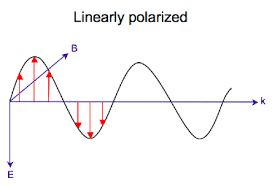
\includegraphics[scale=0.75]{images}
\end{figure}

S polarizacijo opisujemo le transverzalno valovanje, saj pri longitudialnem smer nihanja količine sovpada s smerjo valovanja. Poznamo tri osnovne tipe polarizacije: linearno, krožno in eliptično. [10],[11]

\begin{definicija}
Val je linarno polariziran, če nihanje poteka le v eni smeri. Krožno in eliptično polarizacijo dobimo, kadar se s širjenjem vala nihanje suče. [10],[11]
\end{definicija}

\begin{figure}[h]
\centering
\caption{Osnovni tipi polarizacije}

\includegraphics[scale=2]{polcls}
\end{figure}

Če se smer nihanja neurejeno obrača v vse smeri govorimo o nedoločeni polarizaciji oziroma nepolariziranem valovanju. Takšno je naprimer svetloba, ki jo oddajajo navadna svetila, pa tudi Sonce. [9]

Elektromagnetno valovanje oziroma svetloba je transverzalno valovanje. Sestavljeno iz nihanja električnega in magnetnega polja, ki nihata pravokotno na smer valovanja ter pravokotno en na drugega. Po dogovoru je smer polarizacije enaka smeri nihanja jakosti električnega polja. [10],[11]

V nadaljevanju bomo potrebovali linearno polarizacijo fotonov, zato si poglejmo kako jo lahko umetno ustvarimo. Naj še enkrat opomnimo, da polarizacija fotonov sovpada s polarizacijo elektromagnetnega valovanja. 

\begin{definicija}
Polarizator je naprava, ki valovanje z nedoločeno ali mešano polarizacijo spremeni v valovanje z določeno polarizacijo.
\end{definicija}

\begin{figure}[h]
\centering
\caption{Delovanje polarizatorja}
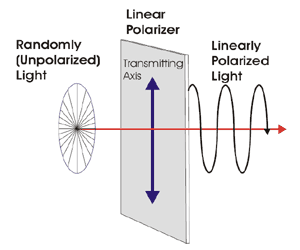
\includegraphics[scale=0.75]{linear-figure-1}
\end{figure}


%KVANTNA RAZDELITEV KLJUČA

\section{Kvantna razdelitev ključa}

\begin{definicija}
Šifriranje podatkov je pretvorba podatkov v tako obliko, da je nepooblaščene osebe ne razumejo. [15]
\end{definicija}

Navadno šifriramo podatke z uporabo algoritmov ter drugih matematičnih postopkov. Čeprav je lahko tak postopek zelo učinkovit in ga morebitni vsiljivci težko dešifrirajo, pa je skoraj nemogoče preveriti prisotnost prisluškovalca. Prav to je izjemna lastnost kvantnega šifriranja podatkov, sogovornika namreč ob koncu pogovora vesta, ali je njuno sporočila prejela še tretja oseba. [16]

Za lažjo razlago postopka poimenujmo našega pošiljatelja sporočila Alica, prejemnika Bob in prisluškovatelja Eva.

Kako torej poteka kvantno šifriranje?
Spoznali smo že fotone in njihovo polarizacijo in izvedeli, kako lahko polarizacijo spreminjamo. Torej lahko z različnimi polarizacijami fotonov predstavimo različne vrednosti. [17]

\begin{zgled}
Naj naprimer linearna polarizacija v smeri y osi ($\uparrow$) v binarnem zapisu pomeni 0, polarizacija v smeri x osi ($\rightarrow$) pa 1. Tako lahko Alica z zaporedjem fotonov, ki jim priredi polarizacijo pošlje Bobu število v binarnem zapisu. [17]
\end{zgled}

Lahko bi definirali še število 2 s polarizacijo v smeri premice pri kotu $45^{\circ}$ ($\nearrow$), ter število 3 pri kotu $135^{\circ}$ ($\nwarrow$) itd., potrebujemo le ustrezni polarizator. Bolj enostavno je, če se omejimo na manjše število polarizacij in uporabimo kvantno šifriranje izključno za pošiljanje ključa, s katerim nato šifriramo nadaljna sporočila. [17]

Bob mora pri prejemu posameznega fotona uporabiti enak polarizator kot ga je Alica pri določanju polarizacije, sicer odčitana vrednost ni nujno pravilna. Navadno za polarizaciji $\uparrow$ in $\rightarrow$ uporabimo polarizator oblike +, za $\nearrow$ in $\nwarrow$ polarizaciji pa polarizator $\times$. Kaj bi se zgodilo, če bi Bob uporabil napačni polarizator pri prejemu fotona? 

\begin{zgled}
Recimo da Alica želi poslati vrednost 1, torej pošlje foton s polarizacijo $\uparrow$. Če Bob namesto polarizatorja +, ki bi pravilno odčital polarizacijo fotona in s tem vrednost uporabi polarizator $\times$, bo naključno prejel eno od $\nearrow$, $\nwarrow$ polarizacij. Torej bo namesto vrednosti 1, prejel število 2 ali 3.
\end{zgled}

Zakaj nam torej tak prenos podatkov omogoča zaznavo prisluškovalca?
Če Eva želi dobiti sporočilo, ki ga Alica pošilja Bobu, mora prestreči poslane fotone, pri tem pa uporabiti enega od polarizatorjev. Eva ne ve katero polarizacijo je Alica izbrala za posamezen foton in lahko le naključno izbere polarizator, s katerim bo prebrala foton in ga nato poslala naprej Bobu. Ima torej 50\% možnosti, da se pri izbiri zmoti, s tem pokvari prvotno polarizacijo in zato Bobu posreduje napačno polariziran foton. Poslano sporočilo se seveda ne bo ujemalo s prejetim in Alica in Bob bosta vedela, da je bila prisotna tudi Eva. 

Pojavi se vprašanje kako naj bi Bob vedel, kateri polarizator mora uporabiti. Alica mu zaradi morebitne prisotnosti Eve seveda ne sme povedati katero polarizacijo je uporabila na fotonih. Odgovor je preprost: tudi Bob ne ve, kateri polarizator mora uporabiti, zato ga kar naključno izbere. Skoraj zagotovo torej Alica in Bob po koncu pošiljanja fotonov tudi brez Eve nimata enakega ključa. Vendar obstaja način, da ga dobita. Pravimo mu BB84 protokol.


%BB84 PROTOKOL

\section{BB84 protokol}


%ZGLED
\section{Prikaz delovanja na zgledu}


%SUDOKU

\section{Sudoku}

\begin{definicija}
Sudoku je logična uganka, pri kateri je cilj zapolniti mrežo velikosti 9x9 s števili od 1 do 9 tako, da se vsako število v vsakem stolpcu, vrstici in 3x3 kvadratu znotraj mreže pojavi natanko enkrat. [3]
\end{definicija}

\begin{figure}[h]
\centering
\caption{Primer rešenega sudokuja}
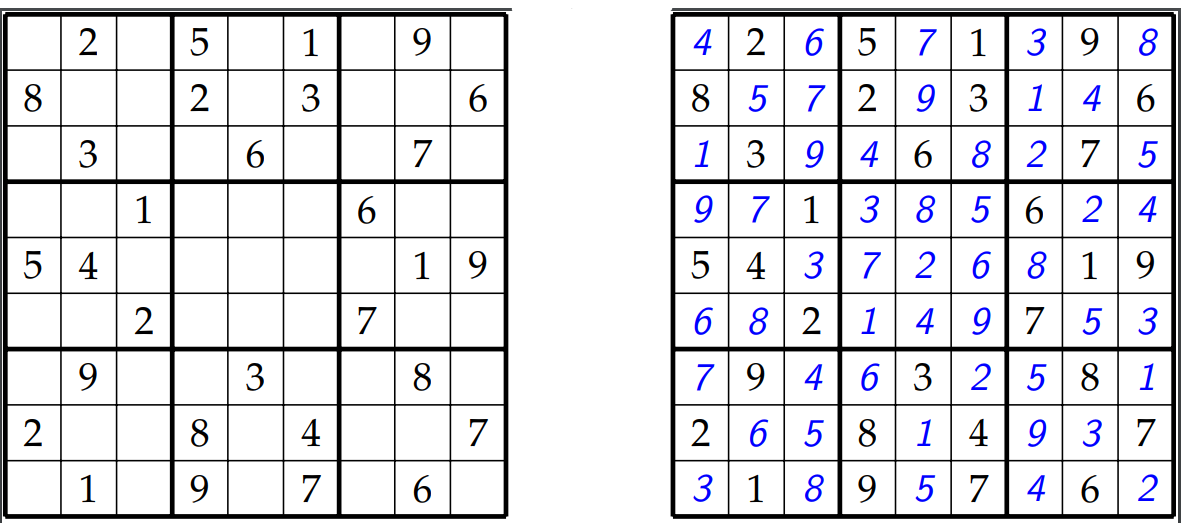
\includegraphics[scale=0.4]{sudoku_resen}
\end{figure}

Sudokuja se je domislil američan Howard Garns in ga prvič objavil leta 1979. Pravijo, da idejo dobil na podlagi Eulerjevega latinskega kvadrata. To je matrika velikosti nxn, napolnjena z n različnimi znaki, pri čemer se vsak znak v vrstici in stolpcu pojavi natanko enkrat. Čez 5 let so uganko objavili tudi na Japonskem in jo poimenovali ''Suuji wa dokushin ni kagiru'', kar v prevodu pomeni ''števke morajo biti edine'', prvi zlogi besed pa nam podajo ravno znano ime uganke: SUDOKU. [3],[4]

%primer latinskega kvadrata na tablo
%poveš da je triljov 10 na 21

Število vseh možnih sudoku mrež, pri velikosti 9x9 je približno 6,6 trilijonov natančneje 6.670.903.752.021.072.936.960. 
Zahtevnost uganke je obratno sorazmerna s številom že vpisanih števil. Lažji sudokuji imajo tako podanih več kot 30 števil, težji pa nekje med 20 in 30. Dolgo je bil odprt problem najmanjšega števila začetnih števil, ki še vedno podajo enolično rešitev. Leta 2012 so dokazali, da je to število 17, saj je bilo iskanje enolične rešitve s pomočjo računalnika za sistem s 16 podanimi števili neuspešno. [3],[4]

Skozi leta so se razvile različne oblike sudokuja in prispevale k težavnosti reševanja. Poznamo naprimer Sudoku X, pri katerem mora poleg standardnih pogojev veljati še, da se števila tudi na diagonalah pojavijo le enkrat. Še bolj ekstremna oblika pa je geometrijski sudoku, pri katerem znotraj mreže nimamo 3x3 kvadratov, temveč različne geometrijske like sestavljene iz devetih polj. [3],[4]

\begin{figure}[h]
\centering
\caption{Geometrijski sudoku}
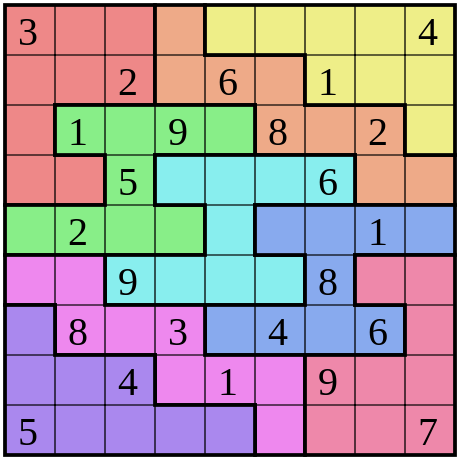
\includegraphics[scale=0.4]{geo_sudoku}
\end{figure}

% SUDOKU KLJUČ

\section{Sudoku ključ}

\end{document}
